% !Mode:: "TeX:UTF-8"

\titlecontents{chapter}[2em]{\vspace{.5\baselineskip}\xiaosan\song}
             {\prechaptername\CJKnumber{\thecontentslabel}\postchaptername\qquad}{} 
             {}                            % 设置该选项为空是为了不让目录中显示页码
\fancypagestyle{plain}   % 设置页眉页脚风格,按照教务处规定,此处出现页眉,但是没有页脚(页码)。
\lhead{}
\rhead{}
% \chead{\song\wuhao 天津大学 2016 届本科生毕业论文} % 设置页眉内容
\lfoot{}

\cfoot{}
\rfoot{}
\markboth{附\quad 录}{附\quad 录}
\addcontentsline{toc}{chapter}{附\quad 录} % 添加到目录中
\chapter*{附\quad 录}
\setcounter{page}{1}

\begin{figure}[htbp!]
    \centering
    \subfigure[n=5000, c=1000]{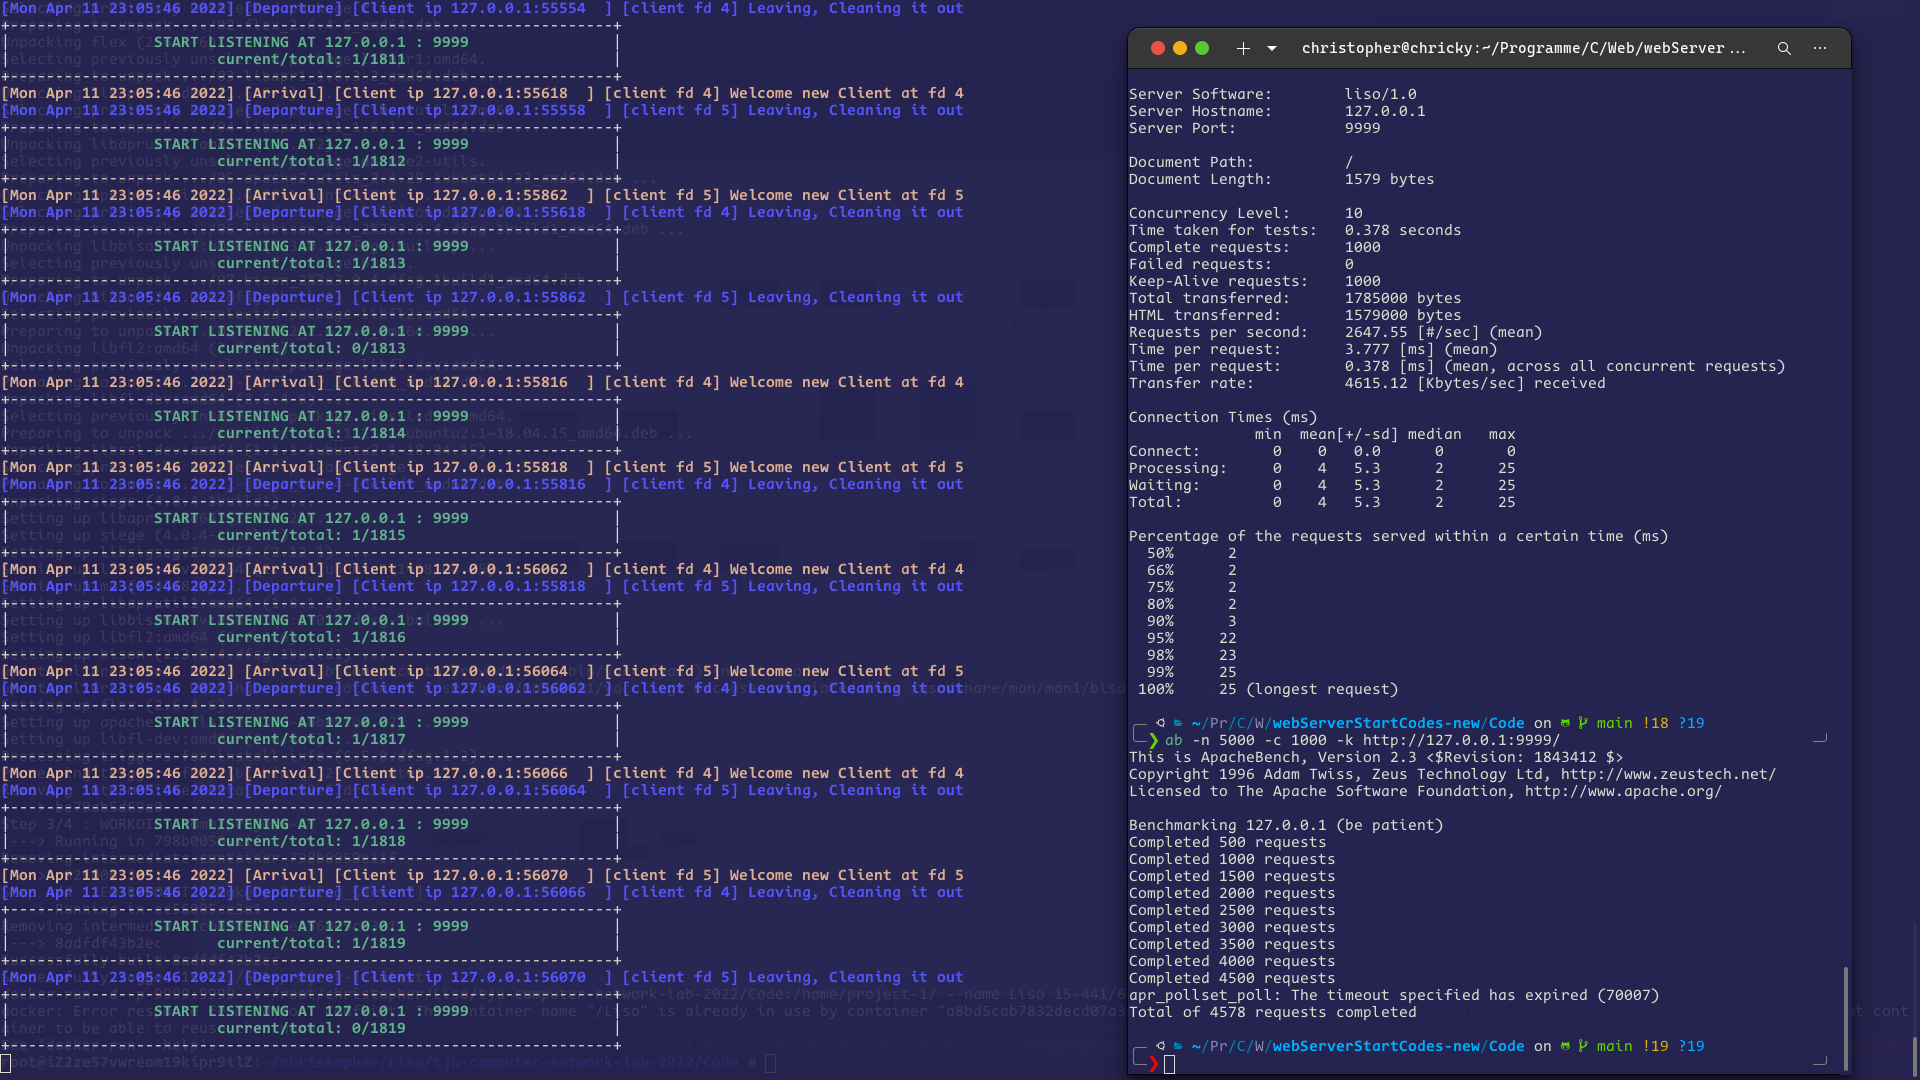
\includegraphics[width=2.6in]{ab5000_1000.png}}
    \subfigure[n=1000, c=100]{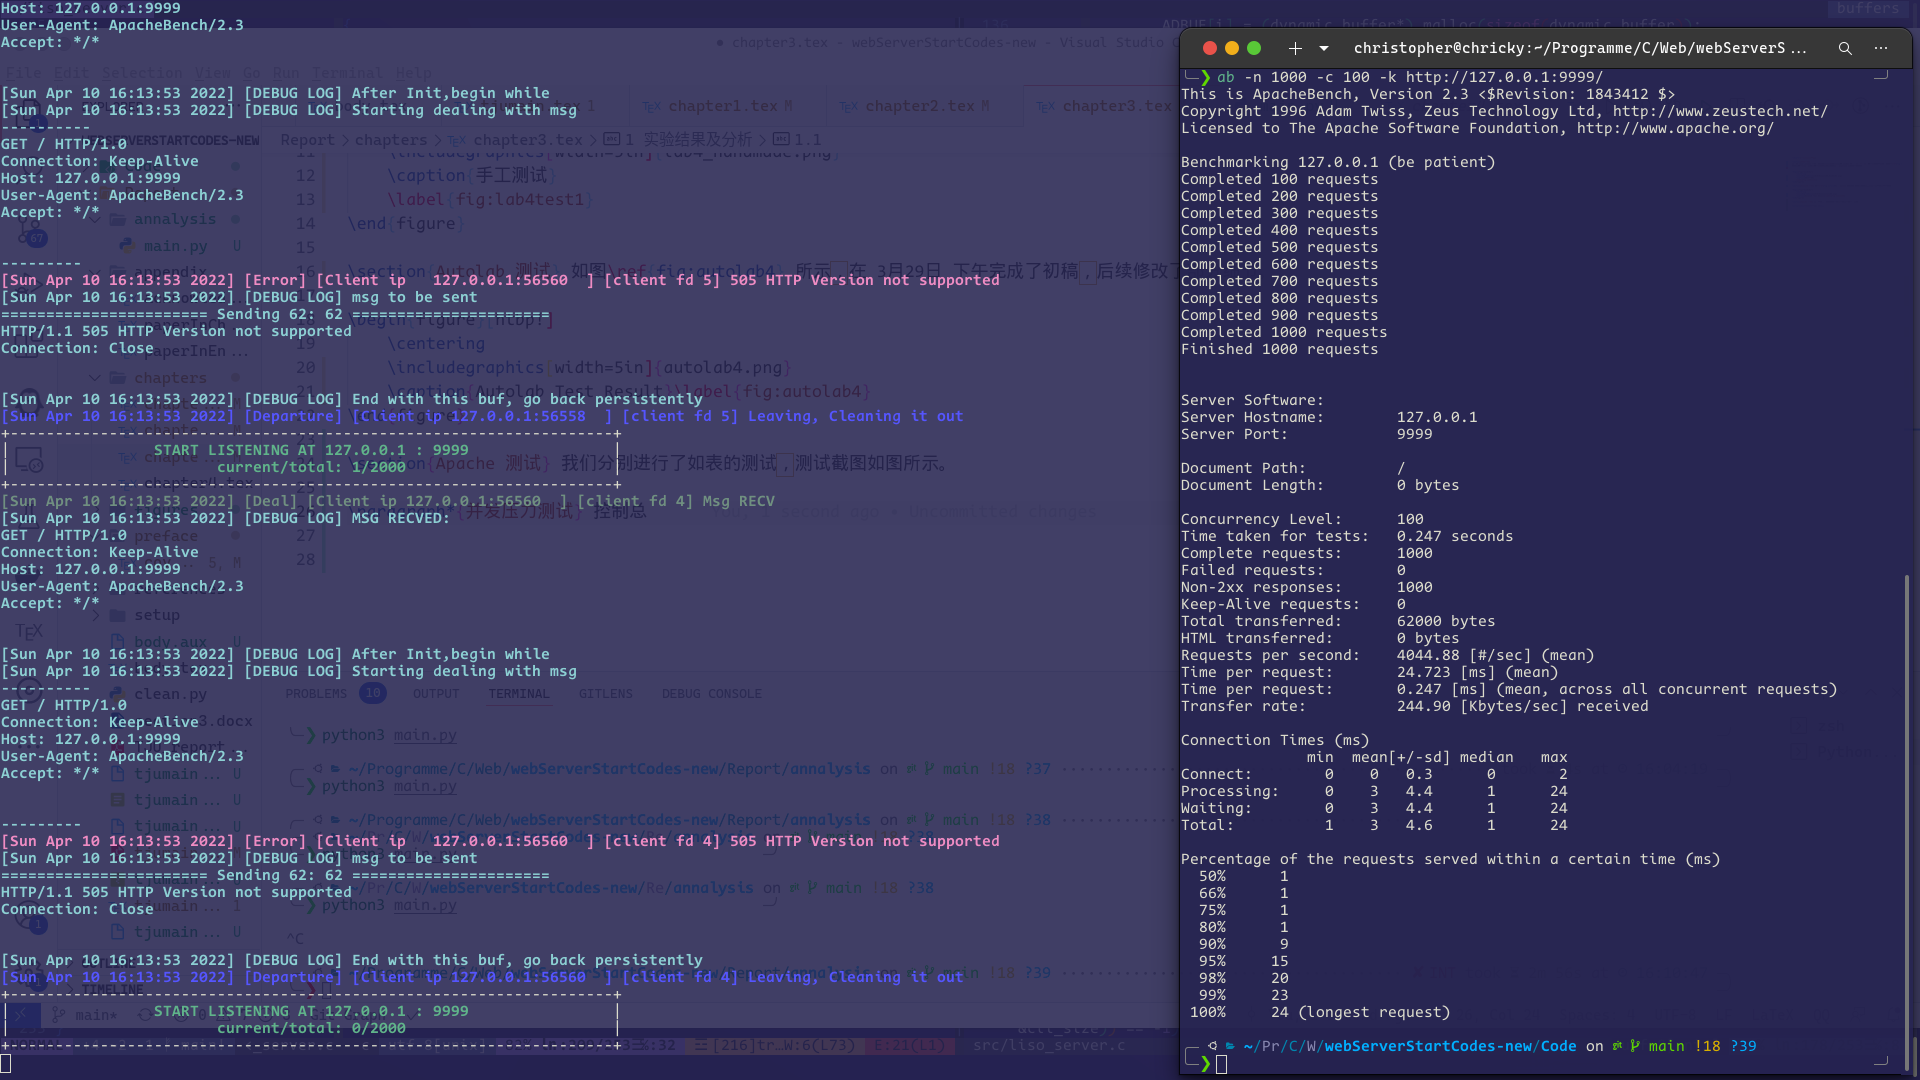
\includegraphics[width=2.6in]{ab1000_100.png}}
    \subfigure[n=1000, c=1000]{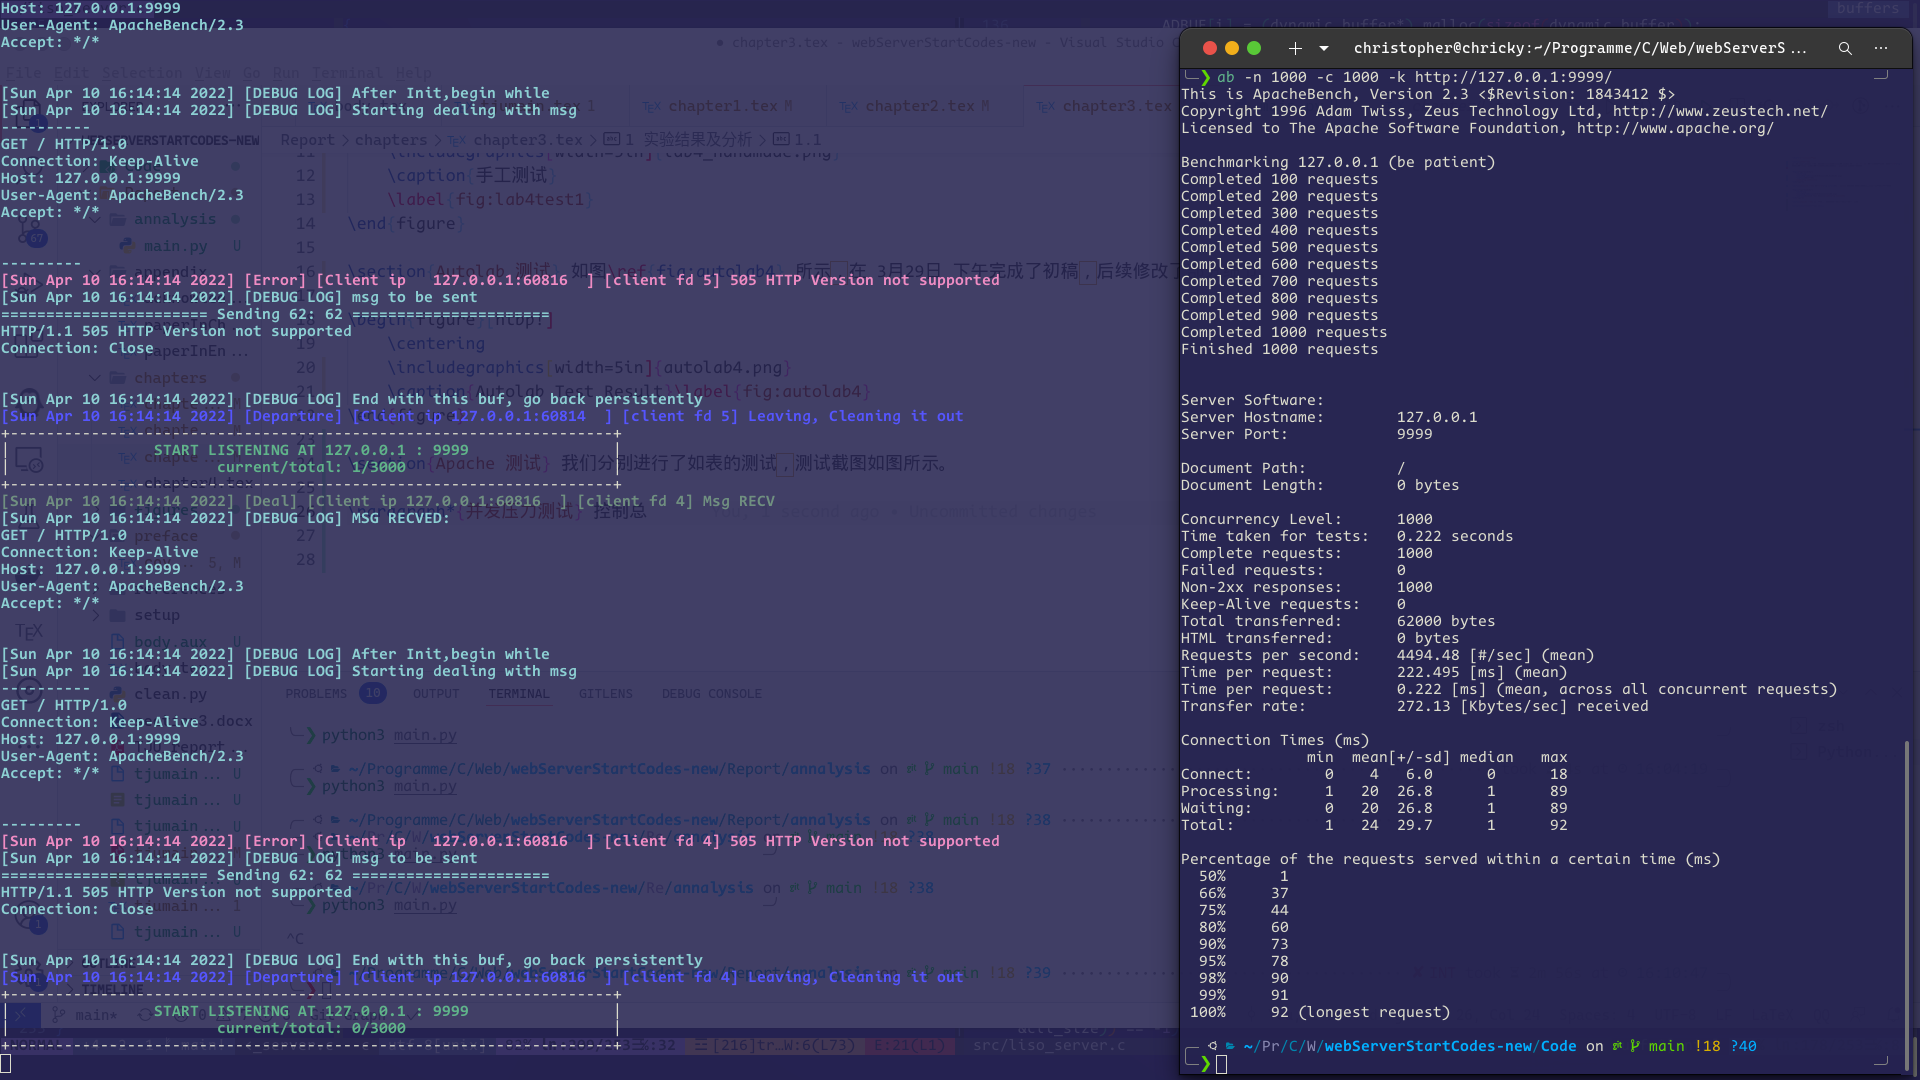
\includegraphics[width=2.6in]{ab1000_1000.png}}
    \subfigure[n=100, c=10]{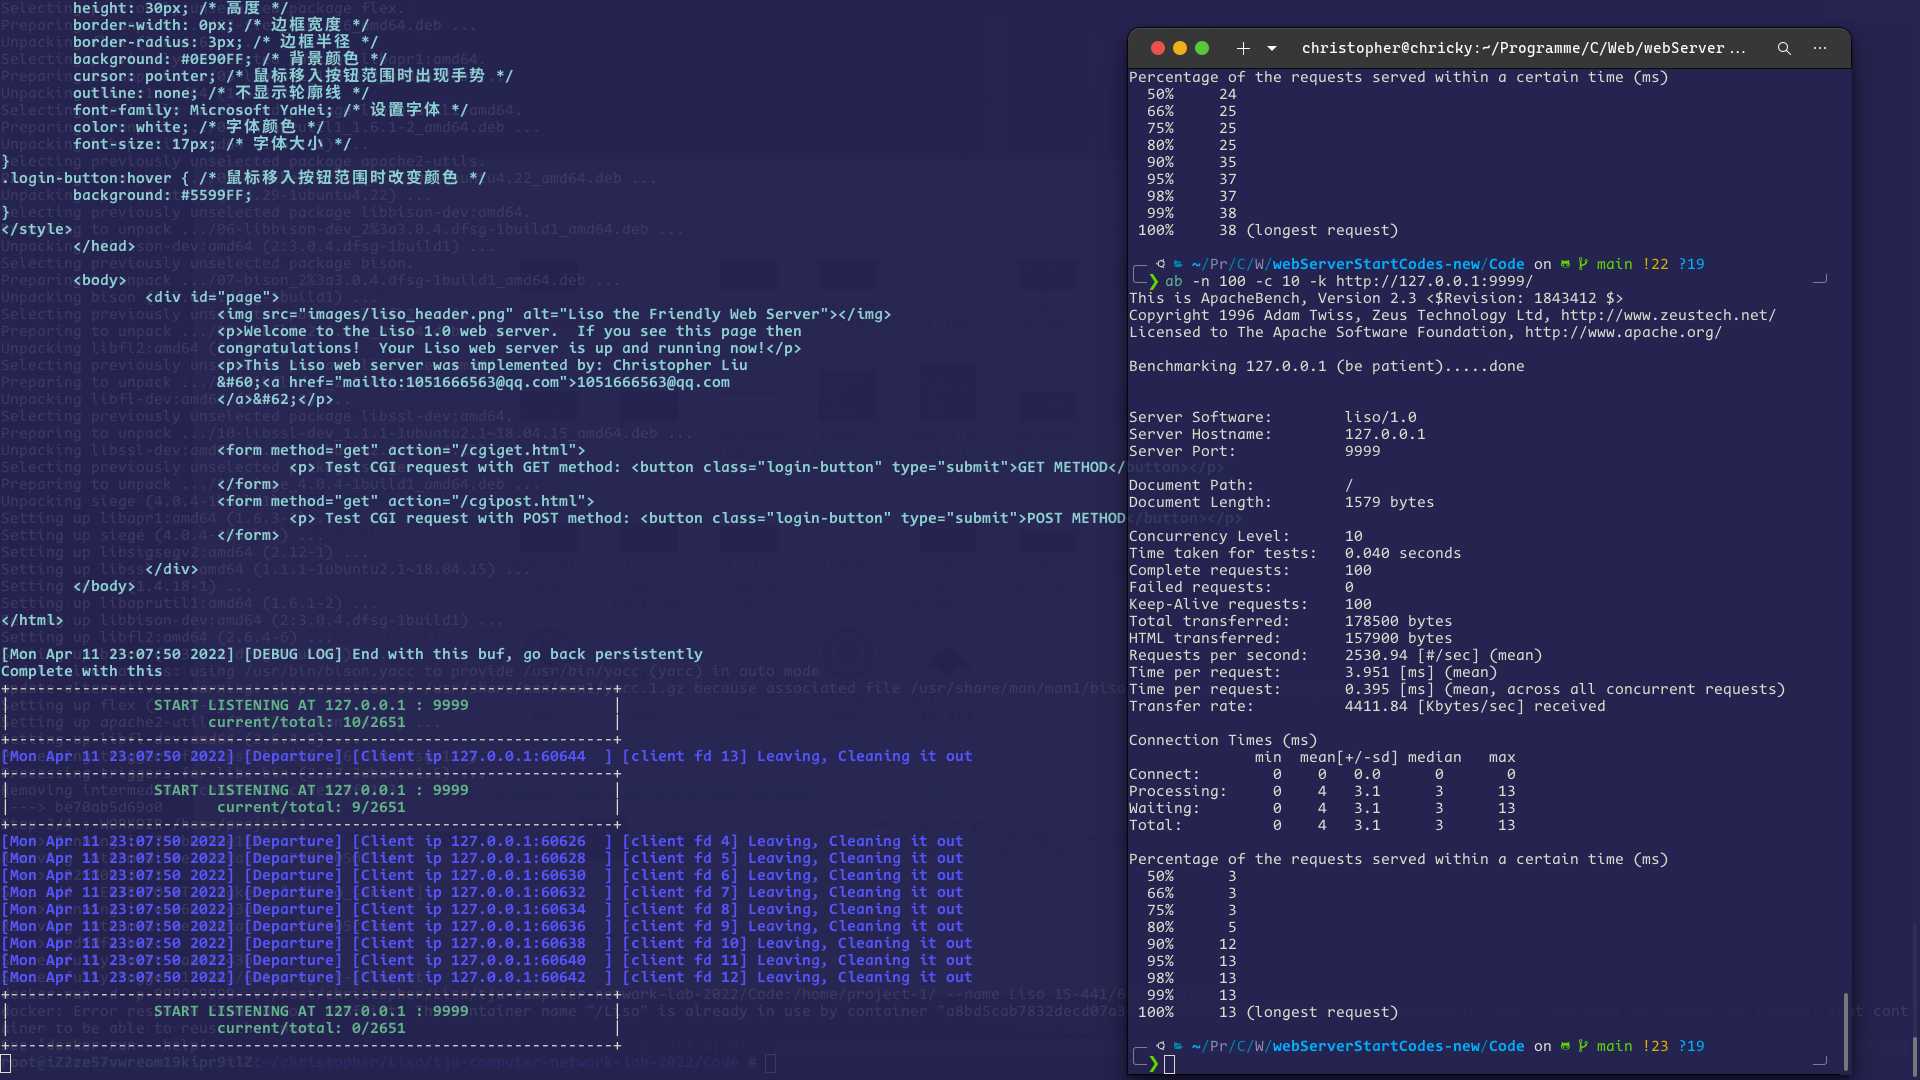
\includegraphics[width=2.6in]{ab100_10.png}}
    \subfigure[n=1000, c=10]{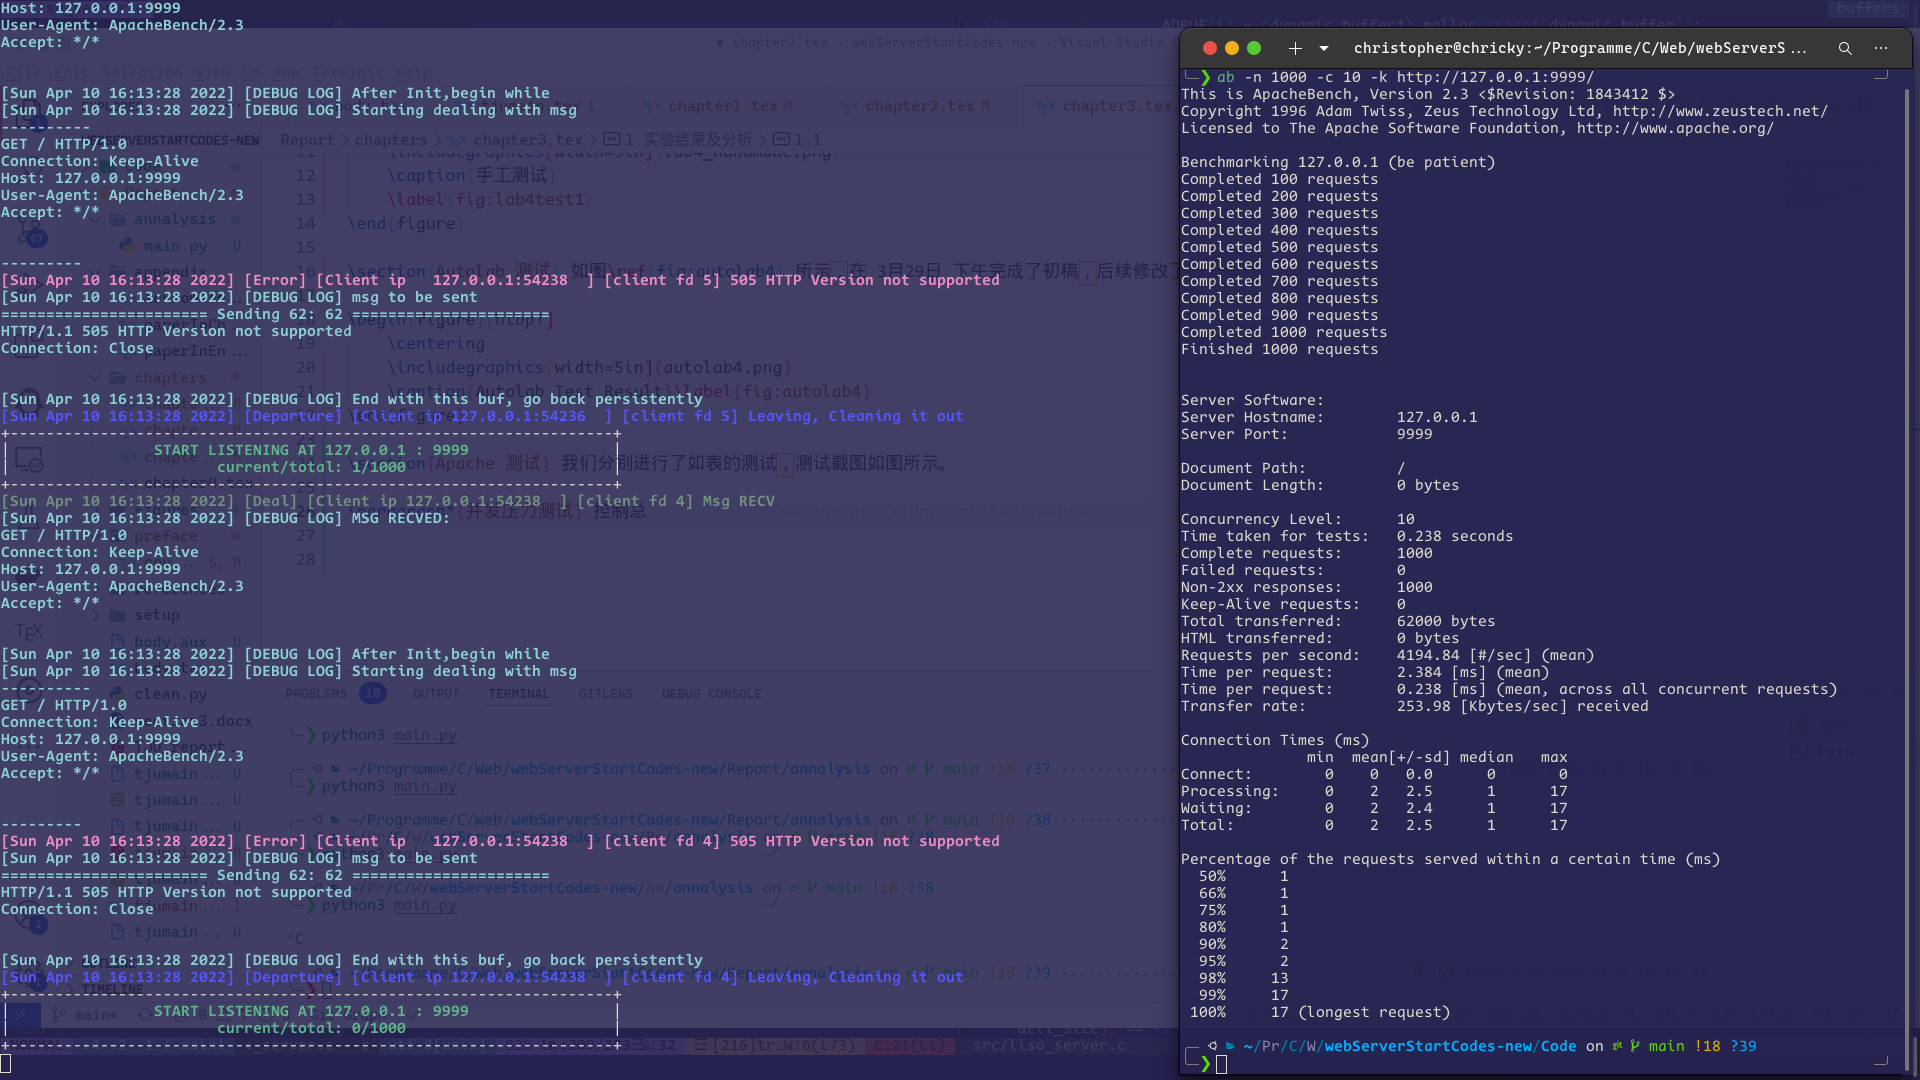
\includegraphics[width=2.6in]{ab1000_10.png}}
    \subfigure[n=10000, c=10]{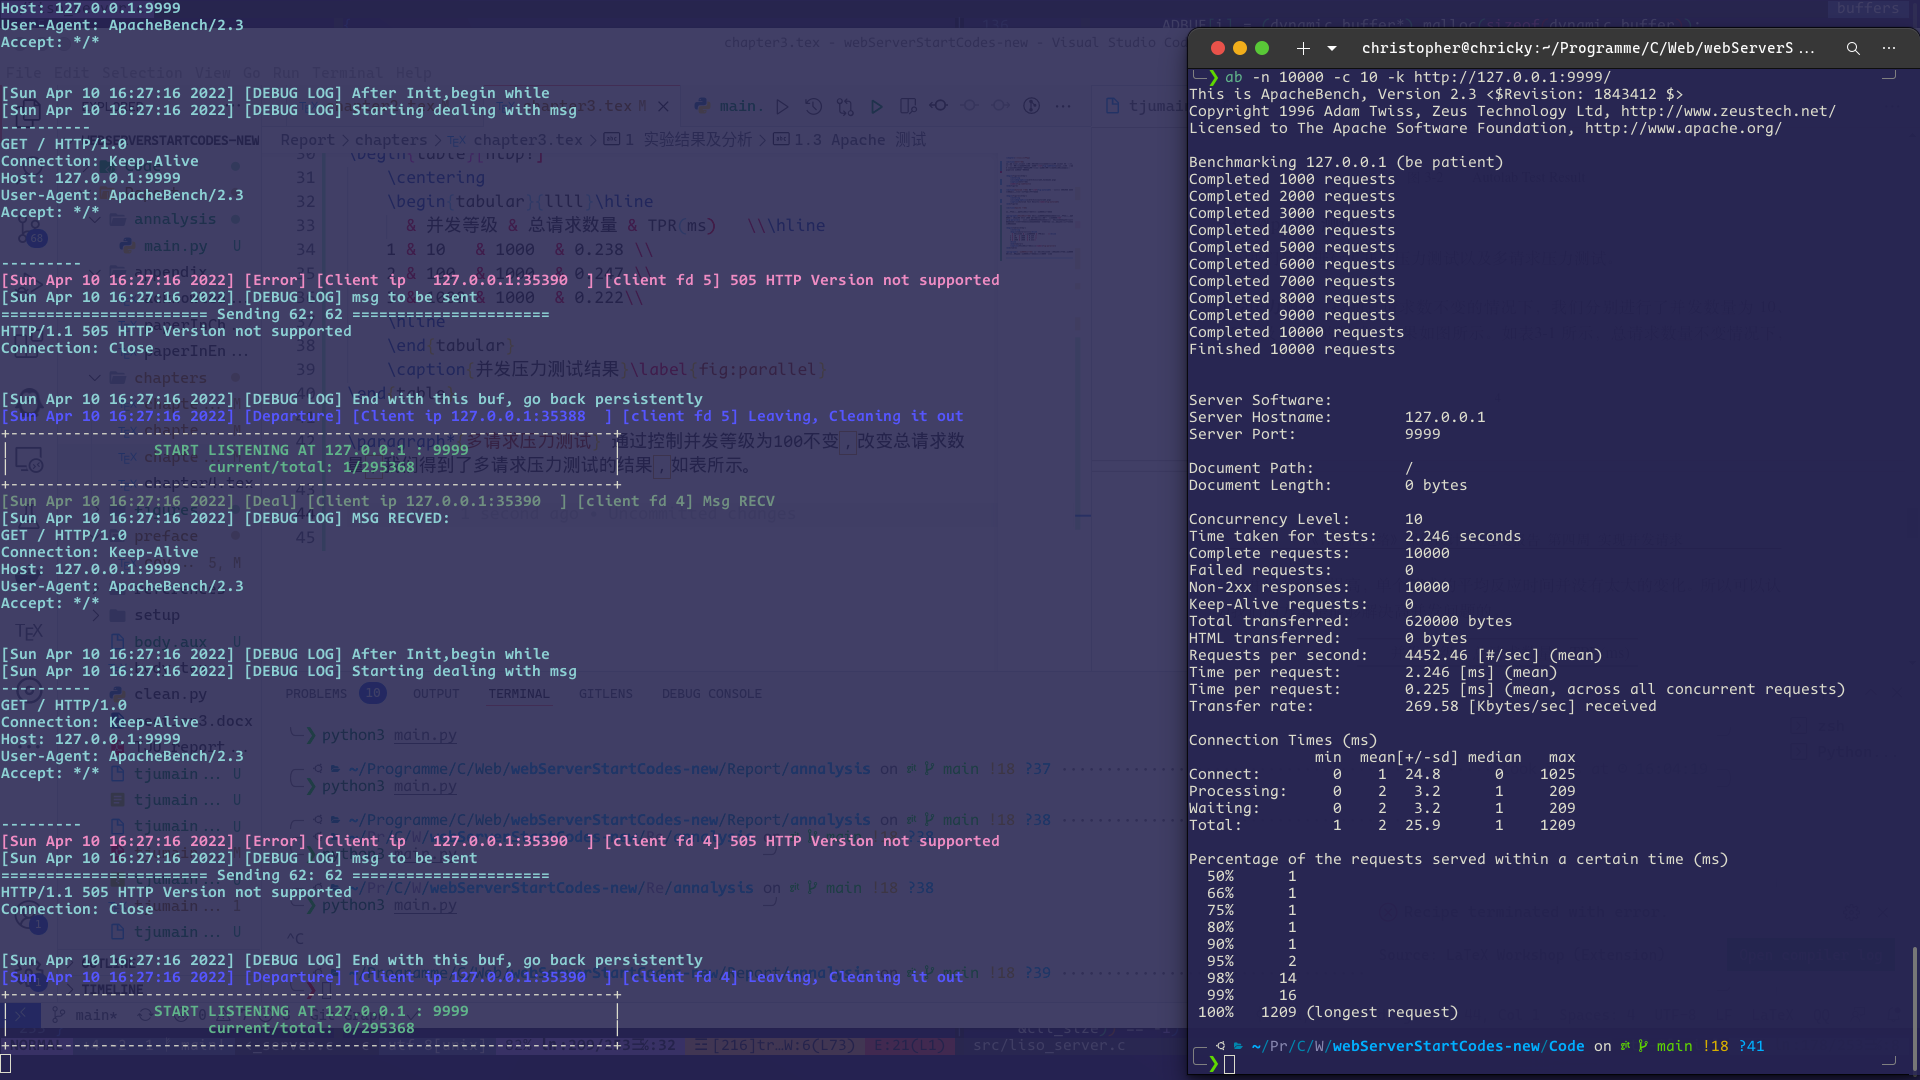
\includegraphics[width=2.6in]{ab10000_10.png}}
    \subfigure[n=100000, c=10]{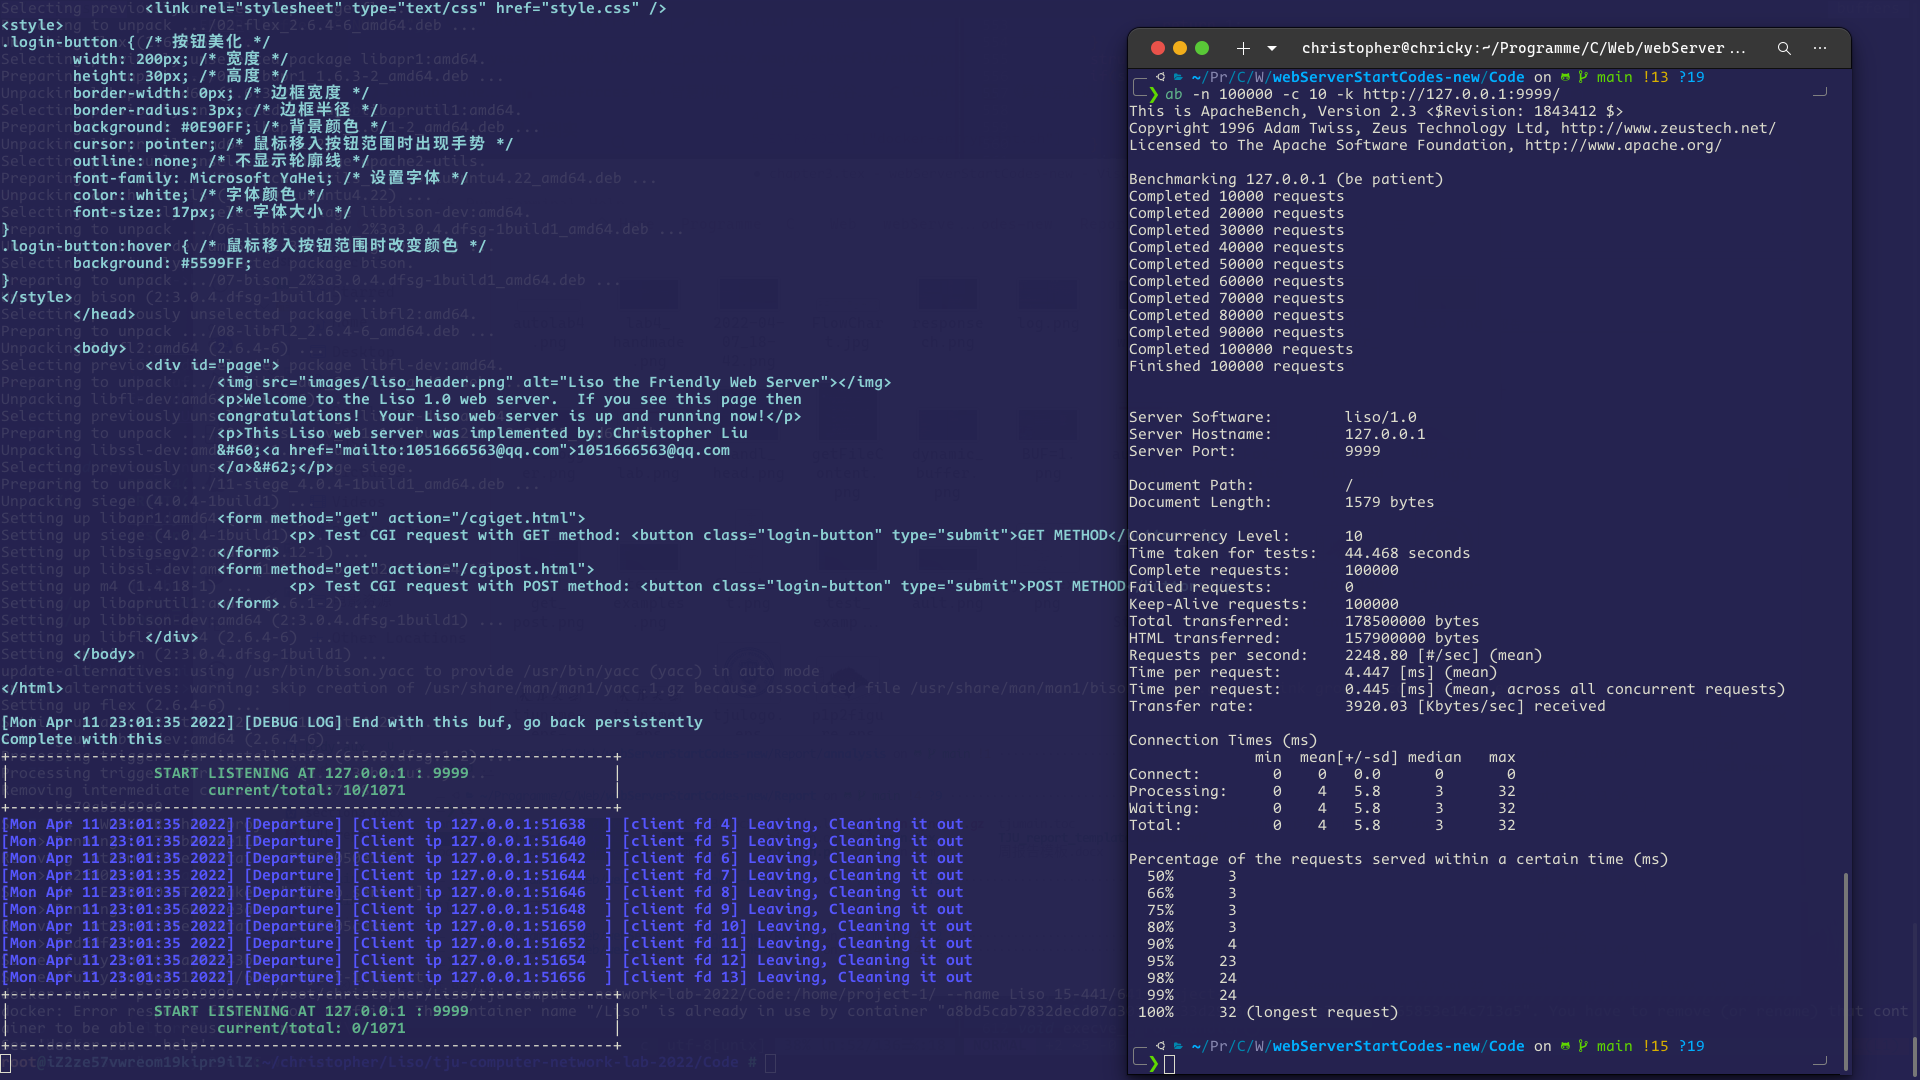
\includegraphics[width=2.6in]{ab100000_10.png}}
    \subfigure[n=1000000, c=10]{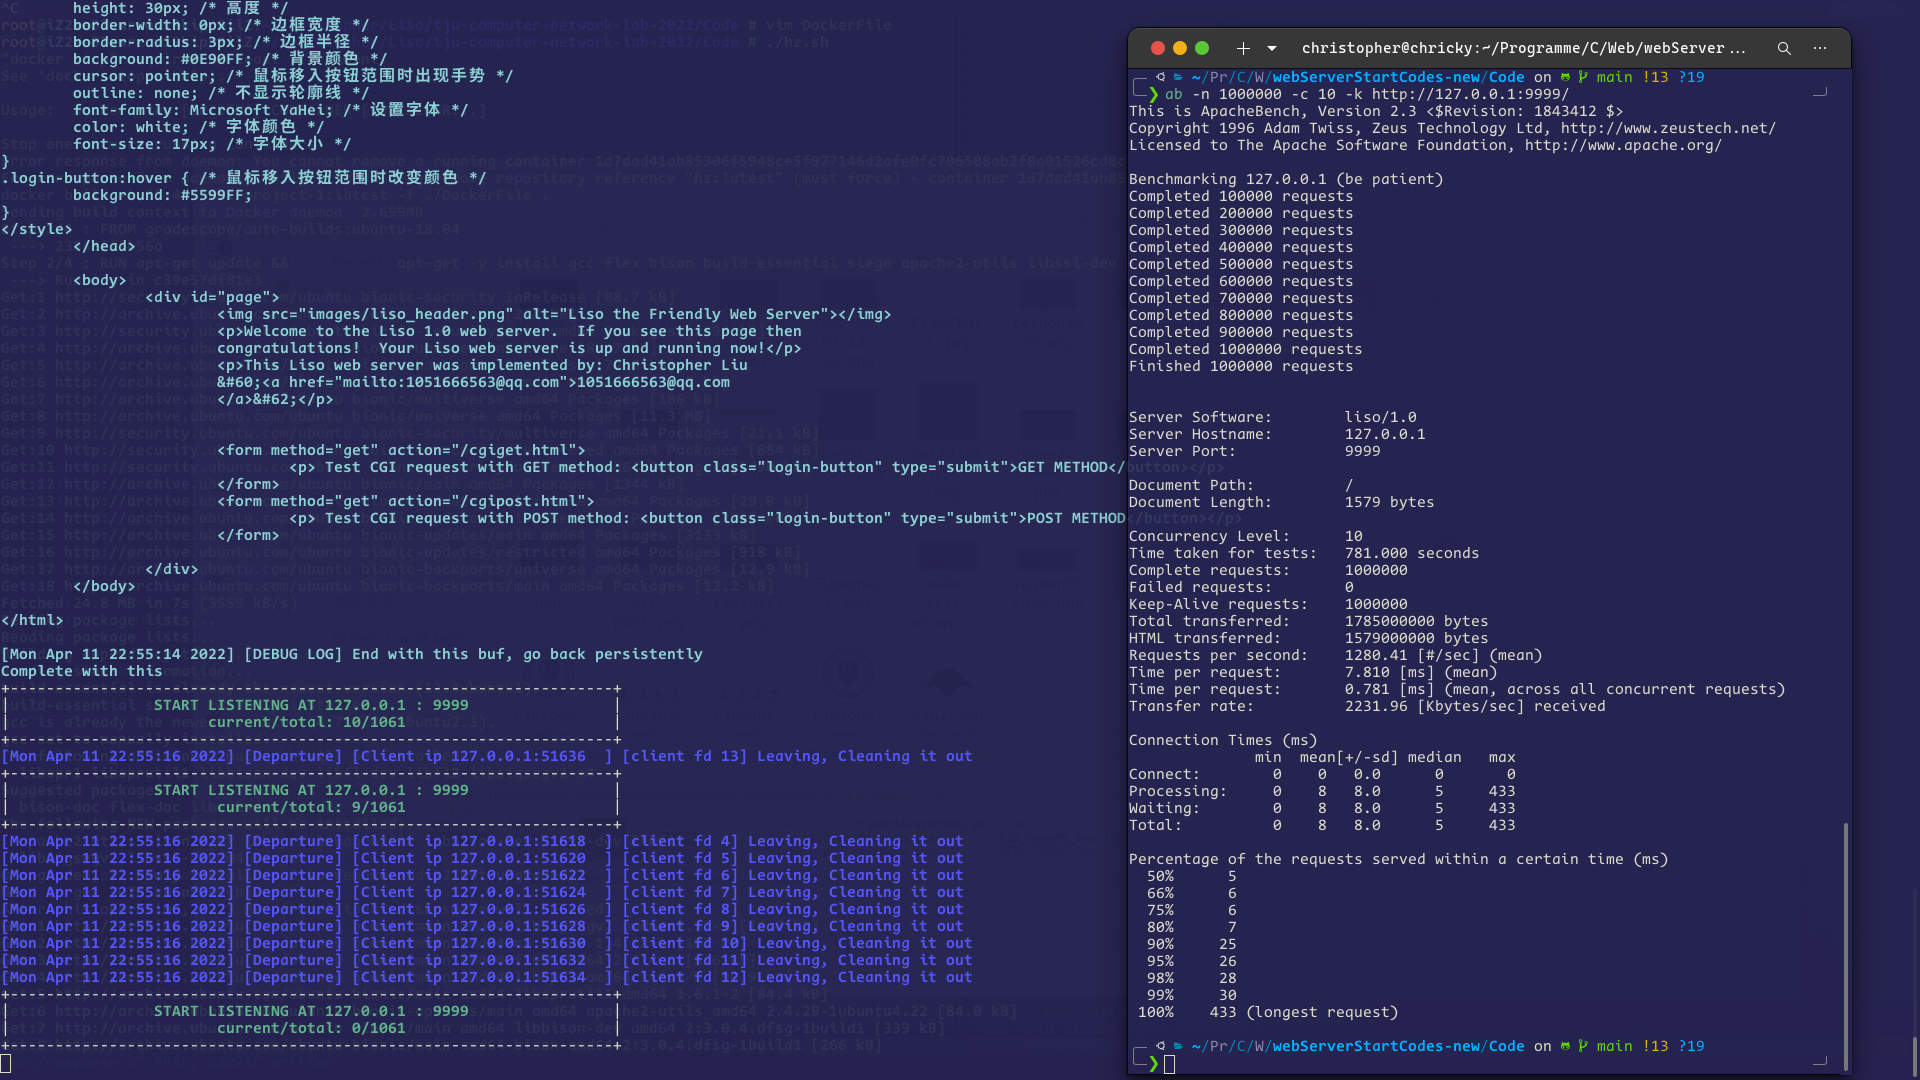
\includegraphics[width=2.6in]{ab1000000_10.png}}
    \caption{Apache Bench 测试}
\end{figure}




